\documentclass{beamer}

% Some common packages
\usepackage{graphicx, color}
\usepackage{alltt}
\usepackage{booktabs, calc, rotating}
\usepackage[round]{natbib}
\usepackage{multicol}
\usepackage{amsmath, amsbsy, amssymb, amsthm, graphicx}
\usepackage[english]{babel}
\usepackage{xkeyval} 
\usepackage{xfrac}
\usepackage[normalem]{ulem}
\usepackage{fancyvrb} 
\usepackage{tikz, geometry, tkz-graph, xcolor}
\usepackage[latin1]{inputenc}
\usepackage{times}
\usepackage[T1]{fontenc}

% Shortcuts
\newcommand{\empr}[1]{{\emph{\color{red}#1}}}
\newcommand{\cov}{\mathrm{cov}}
\newcommand{\pkg}[1]{{\textbf{\texttt{#1}}}}
\newcommand{\dif}{\mathrm{d}}
\newcommand{\bigbrk}{\vspace*{2in}}
\newcommand{\smallbrk}{\vspace*{.1in}}
\newcommand{\midbrk}{\vspace*{1in}}
\newcommand{\red}[1]{{\color{red}#1}}
\newcommand{\blue}[1]{{\color{blue}#1}}
\newcommand{\green}[1]{{\color{green}#1}}
\newcommand{\calc}[1]{{\fbox{\mbox{#1}}}}
\newcommand{\Var}{\mathrm{Var}}%
\newcommand{\Cov}{\mathrm{Cov}}%

\mode<presentation>
{
	\usetheme{UTD}
	\usecolortheme[RGB={200,0,0}]{structure}
	\setbeamercovered{transparent}
}

% fancy for Verbatim?
\fvset{frame=single,framesep=1mm,fontfamily=courier,fontsize=\scriptsize,numbers=left,framerule=.3mm,numbersep=1mm,commandchars=\\\{\}}


\title[Survival Analysis]{Applied Survival Analysis Using R\\ Chapter 5: Regression Analysis Using the Proportional Hazards Model}
\author[Qi Guo]{Qi Guo}
\institute[UTD]{Department of Mathematical Sciences \\ 
	The University of Texas at Dallas}
\date{April, 12 2019}
	
\begin{document}

\begin{frame}
  \titlepage
\end{frame}

% Set up UTD backgroud
\setbeamercolor*{item}{fg=red}
\bgroup
\usebackgroundtemplate{
\tikz[overlay,remember picture] \node[opacity=0.05, at=(current page.center)] {
   
\includegraphics[height=\paperheight,width=\paperwidth]{UTDbg}};}


\section[Outline]{}
\begin{frame}
  \tableofcontents
\end{frame}

\section{Covariates and Nonparametric Survival Models}
\begin{frame}
\frametitle{Covariates}
\begin{defblock}{Covariate}
In general terms, \empr{covariates} are characteristics (excluding the actual treatment) of the participants in an experiment. If you collect data on characteristics before you run an experiment, you could use that data to see how your treatment affects different groups or populations. It uses in \empr{ANCOVA}
\end{defblock}
Characteristics:
\begin{itemize}
\item A covariate can be an \empr{independent variable} or it can be an unwanted, confounding variable. Adding a covariate to a model can increase the accuracy of your results.
\item Observed/measured (as opposed to a manipulated variable).
\item A control variable.
\end{itemize}
\end{frame}

\pagebreak
\begin{frame}
\frametitle{The proportional hazards model}
\begin{itemize}
\item Proportional hazard function: 
\begin{equation}
h_1(t)={\psi}h_0(t)
\end{equation}
\item Furthermore, we can extend the model to include {\color{red}covariate} information in a vector $z$ as follows:
\begin{equation}
{\psi}=e^{z\beta}
\end{equation}
\item \empr{Partial likelihood} for assuming a form for $h_0(t)$.
\end{itemize}
\end{frame}

\section{Comparing Two Survival Distributions Using a Partial Likelihood Function}
\begin{frame}
\frametitle{The partial likelihood}
\begin{itemize}
\item The partial likelihood will allow us to use an unspecified \empr{baseline survival distribution} to define the survival distributions of subjects based on their covariates.
\item Why partial likelihood?
\begin{itemize}
\item It is a product of expressions, one for each failure time, while censoring times do not contribute any factors.
\item The factors of a partial likelihood are {\color{red}conditional probabilities}.
\end{itemize}
\end{itemize}
\end{frame}

\pagebreak
\begin{frame}
\frametitle{Notation}
\begin{itemize}
\item The hazard function for Subject $i$ at failure time $t_j$ is $h_i(t_j)$.
\item $j$ denotes the $j'th$ failure time (where the failure times are sorted from lowest to highest)
\item Under the proportional hazards model,write this hazard function as: 
\begin{itemize}
\item $h_i(t_j)=h_0(t_j){\psi_i}$
\item ${\psi_i}=e^{z_i\beta}$
\item Covariate $z_i$ is either \empr{1} (if the patient is in the {\color{red}experimental group}) or \empr{0} (of the patient is in the {\color{red} control group})
\end{itemize}
\item Patients in the experimental group are expected less likely than control patients to experience the event(experiment work expected)
\begin{itemize}
\item $\beta < 0$ and $\psi < 1$.
\end{itemize}
\item {\color{red}$\psi_i = 1$ if a patient is in the control group} or {\color{red} $\psi_i=\psi$ if a patient is in the experimental group}.
\end{itemize}
\end{frame}

\pagebreak
\begin{frame}
\frametitle{Formula}
\begin{itemize}
\item The first failure time $t_1$.The set of all subjects in the trial ``\pkg{at risk}'' for failure is denoted by $R_1$(Before the first failure, all of the patients in ``\pkg{at risk}'' ).
\item Among them in $R_1$, the probability that Patient $i$ fails in the hazard, $h_i(t_j)=h_0(t_j){\psi_i}$, for that patient divided by the sum of the hazards of all of the patients:
\begin{equation}
p_1 = \frac{h_i(t_1)}{\sum\limits_{k\in R_1}^{}h_k(t_1)} = \frac{h_0(t_1)\psi_i}{\sum\limits_{k\in R_1}^{}h_0(t_1)\psi_k}
\end{equation}
\item where {\color{red}$h_0(t_1)$} is the hazard for a subject from the control group, and is that the \empr{baseline hazard function}.
\item Cancels out, we have: 
\begin{equation}
p_1 = \frac{\psi_i}{\sum\limits_{k\in R_1}^{}\psi_k}
\end{equation}
\end{itemize}
\end{frame}

\pagebreak
\begin{frame}
\frametitle{Example}
\begin{itemize}
\item The partial likelihood:
\begin{equation}
L(\psi) = p_1p_2\cdots p_D
\end{equation}
\begin{figure}[h!]
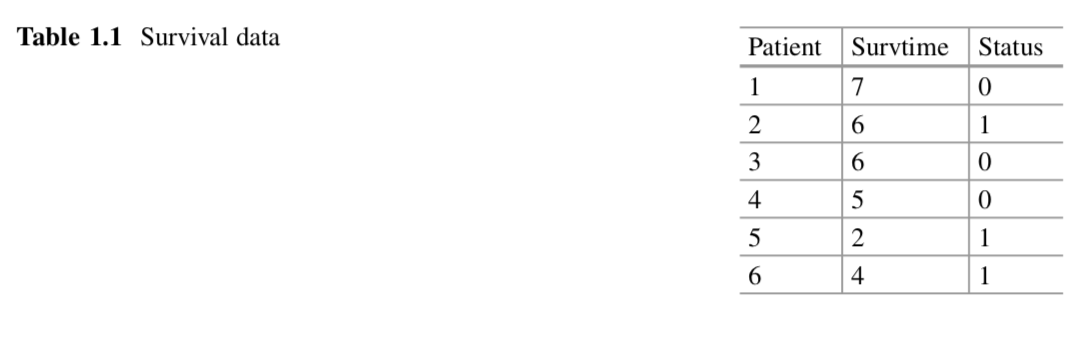
\includegraphics[scale = .5]{001.png}
\end{figure}
\item We know $\psi_1 = \psi_2 = \psi_4 =1$ and $\psi_3 = \psi_5 = \psi_6 = \psi$, substituting into (4), at time 6, a control patients failure, 3 control and 3 treated at risk.
\begin{equation}
	p_1 = \frac{1\cdot h_0(t_1)}{3\cdot h_0(t_1)\psi +3\cdot h_0(t_1)} = \frac{1}{3\psi+3} 
\end{equation}
\end{itemize}
\end{frame}

\pagebreak
\begin{frame}
\frametitle{Example}
\begin{itemize}
\item The second failure time, $t = 10$:
\begin{equation}
p_2 = \frac{\psi}{3\psi+1} 
\end{equation}
\item The third failure time, $t = 15$:
\begin{equation}
p_3 = \frac{1}{2\psi+1} 
\end{equation}
\item The last failure time, $t = 25$ only one subject at risk and died, so it just 1:
\item  The partial likelihood:
\begin{equation}
L(\psi) = \frac{\psi}{(3\psi+3)(3\psi+1)(2\psi+1)}
\end{equation}
\end{itemize}
\end{frame}

\pagebreak
\begin{frame}[fragile]
\frametitle{Transformation}
\begin{itemize}
\item Let $\psi=e^{\beta}$,and take a derivative:
\begin{equation}
\ell(\beta) = \beta - \log(3e^{\beta}+3) - \log(3e^{\beta}+1) -  \log(2e^{\beta}+1)
\end{equation}
\item {\color{red}The maximum partial likelihood estimate} is the value of that \empr{maximizes} this function.
\item Defining the function $\ell(\beta)$:
\begin{Verbatim}
>plsimple <- function(beta) \{
psi <- exp(beta)
result <- log(psi)-log(3*psi+3)-log(3*psi+1)-log(2*psi+1) result\}
\end{Verbatim}
\item Find the {\color{red}m.p.l.e} (maximum partial likelihood estimate) using the  ``\texttt{optim}'' function(In my \texttt{R for data science} presentation).
\begin{Verbatim}
>result <- optim(par=0, fn = plsimple, method = "L-BFGS-B",
control=list(fnscale = -1),lower = -3, upper = 1)
>result$par
[1] -1.326129
\end{Verbatim}
\item Thus, the {\color{red}m.p.l.e} is $\hat{\beta}=-1.326129$.
\end{itemize}
\end{frame}

\section{The Partial Likelihood Hypothesis Tests}
\begin{frame}
\frametitle{Recall}
\begin{itemize}
\item Test of $H_0: \beta=0$
\item The \empr{score} function: $S(\beta) = \ell'(\beta)$
\item The \empr{information} function: $I(\beta) = -S'(\beta) = -\ell''(\beta)$, and the second derivative $-\ell''(\beta)$ is also known as the \empr{Hessian}.
\item Three  forms of test:	
\begin{itemize}
	\item \empr{The Wald test}
	\item The score test
	\item  \empr{The likelihood ratio test}
\end{itemize}
\end{itemize}
\end{frame}

\pagebreak
\begin{frame}
\frametitle{The Wald Test}
\begin{itemize}
\item \empr{The Wald test} is perhaps the most commonly used test.
\item The test form $Z = \hat{\beta}/s.e(\hat{\beta})$
\begin{itemize}
\item $\hat{\beta}$ was the value of $\beta$ that maximizes $\ell(\beta)$.
\item  $s.e(\hat{\beta}) = 1/\sqrt{I(\hat{\beta})}$
\item  Construct a normalized test statistic $Z_w = \hat{\beta}/s.e(\hat{\beta})$
\end{itemize}
\item Reject $H_0: \beta=0$ if $|Z_w| > z_{\alpha/2}$
\item Equivalently, Reject $H_0: \beta=0$ if $Z _{w}^{2} > \chi _{\alpha,1}^{2}$
\item Construct a $1-\alpha$ confidence interval: $\hat{\beta}\pm z_{\alpha/2}\cdot s.e.(\hat{\beta})$.
\end{itemize}
\end{frame}

\pagebreak
\begin{frame}
\frametitle{The Score Test}
\begin{itemize}
\item The test form $Z_s = S(\beta = 0)/\sqrt{I(\beta = 0)}$
\begin{itemize}
 \item Reject $H_0: \beta=0$ if $|Z_s| > z_{\alpha/2}$
	\item Equivalently, Reject $H_0: \beta=0$ if $Z _{s}^{2} > \chi _{\alpha,1}^{2}$
\end{itemize}
\item \empr{The score test} is equivalent to the {\color{red}log-rank test}, as we saw in the previous section. This test can be carried out without finding the maximum likelihood estimate $\hat{\beta}$.
	\end{itemize}
\end{frame}

\pagebreak
\begin{frame}
\frametitle{The Likelihood Ratio Test}
\begin{itemize}
\item The likelihood ratio test uses the result \empr{ $2[\ell(\beta=\hat{\beta}) - \ell(\beta=0)]$} follows approximately a chi-square distribution with one df.
\item The key {\color{red}advantage} of this test over the other two is that it is invariant to monotonic transformations of $\beta$.
\end{itemize}
\begin{problock}{Example}
We illustrate these three tests using the simple data last Example, begin by presenting the output from the  ``\texttt{coxph}'' function. The result is put into a data structure called ``\texttt{result.cox}'', and a complete summary of the results we obtain using the ``\texttt{summary}'' function.
\end{problock}
\end{frame}

\pagebreak
\begin{frame}[fragile]
\frametitle{\texttt{coxph} function}

\begin{Verbatim}
>result.cox <- coxph(Surv(tt,status) ~ grp)
>summary(result.cox)
[1] Call:  coxph(Surv(tt,status) ~ grp)
      
      n = 6, number of events= 4
     
         coef       exp(coef)     se(coef)       z      Pr(>|z|)
grp    -1.3261       0.2655        1.2509      -1.06      0.289
         exp(coef)  exp(-coef)    lower.95    upper.95
grp       0.2655      3.766        0.02287      3.082
Concordance= 0.7 (se = 0.187)
Rsquare= 0.183 (max possible=0.76)
Likelihood ratio test= 1.21 on 1 df, p=0.2715
Wald test            = 1.12 on 1 df, p=0.2891
Score (logrank) test = 1.27 on 1 df, p=0.2591
\end{Verbatim}
\end{frame}

\pagebreak
\begin{frame}[fragile]
\frametitle{Without \texttt{coxph} function}
\begin{itemize}
\item The Score test
\begin{Verbatim}
>library(numDeriv)
>grad(func=plsimple, x=0) #The score evaluated at beta = 0 numerically using
the ``gradient'' function
[1] -0.917
>hessian(func=plsimple, x=0) #The information
   [,1] [1,] -0.660
\end{Verbatim}
\item So the $Z_{s}^{2} = (-0.917)^{2}/0.660 = 1.274$
\item And the test \empr{p-value} is given by the upper tail:
\begin{Verbatim}
>pchisq(1.274, df=1, lower.tail=F)
[1] 0.259
\end{Verbatim}
\end{itemize}
\end{frame}

\pagebreak
\begin{frame}[fragile]
\frametitle{Without \texttt{coxph} function}
\begin{itemize}
\item The Wald test
\item Before we get $\hat{\beta} = -1.326129$, and need information to get s.e:
\begin{Verbatim}
>hessian(func=plsimple, x=result.cox$par)
      [,1]
[1,] -0.639
>sqrt(1/0.639) #s.e
[1] 1.251
\end{Verbatim}
\item Finally, the Wald test statistic $Z_w$ and two-sided p-value for the test are given by:
\begin{Verbatim}
>-1.326/1.251
[1] -1.060
>2*pnorm(1.060, lower.tail=F) 
[1] 0.289
\end{Verbatim}
\end{itemize}
\end{frame}

\pagebreak
\begin{frame}[fragile]
\frametitle{Without \texttt{coxph} function}
\begin{itemize}
\item The partial likelihood ratio test
\item The likelihood ratio statistic is twice the difference in the log partial likelihoods evaluated at $\hat{\beta}$ and at 0:
\begin{Verbatim}
>betahat <- result.cox$par
>2*(plsimple(betahat) - plsimple(0))
[1] 1.209
\end{Verbatim}
\item Along with the \texttt{p-value} derived from the \texttt{chi-square} distribution:
\begin{Verbatim}
>pchisq(1.209, 1, lower.tail=F)
[1] 0.271
\end{Verbatim}
\item Besides, the statistic ``\texttt{r-squared}'' is an adaptation to survival analysis of the $R^2$ statistic from linear regression:
\begin{equation}
R^2 = 1 - (\frac{\ell(0)}{\ell(\hat{\beta})})^{2/n}  
\end{equation}
\end{itemize}
\end{frame}

\section{Baseline Survival Function}
\begin{frame}
\frametitle{Baseline Survival Function}
\begin{itemize}
\item An estimate of the \empr{baseline hazard function} is given by:
\begin{equation}
h_0(t_i) = \frac{d_i}{\sum\limits_{j\in R_i}{} exp(z_j\hat{\beta})}
\end{equation}
\item An estimate of the \empr{baseline survival function} is given by:
\begin{equation}
S_0(t) = exp[-H_0(t)]
\end{equation}
\item To find a survival curve for a particular covariate value $z$ use:
\begin{equation}
S(t|z) = [S_0(t)]^{exp(z\hat{\beta})}
\end{equation}
\item In \texttt{R} the ``\texttt{basehaz}'' function will compute a cumulative baseline hazard function, use the option ``\texttt{entered = F}'' to cause it to estimate the cumulative hazard at $\beta = 0$
\end{itemize}
\end{frame}


\section{Left Truncation}
\begin{frame}[fragile]
\frametitle{Example 1}
\begin{itemize}
\item Enter the data as before(Chapter 3):
\begin{Verbatim}
>tt <- c(6, 7, 10, 15, 19, 25)
>status <- c(1, 0, 1, 1, 0, 1)
>grp <- c(0, 0, 1, 0, 1, 1)
>backTime <- c(-3, -11, -3, -7, -10, -5)
\end{Verbatim}
\item Without {\color{red}Left Truncation}
\begin{Verbatim}
>coxph(Surv(tt, status) ~ grp)
     coef    exp(coef)    se(coef)    z       p 
grp -1.33       0.266       1.25    -1.06    0.29

Likelihood ratio test=1.21 on 1 df,p=0.271 n= 6,number 
of events= 4
\end{Verbatim}
\item Conclusion: The experimental group has a \empr{lower hazard} than the control group, but this difference is \empr{not statistically significant}(p-value = 0.271 based on the likelihood ratio test).
\end{itemize}
\end{frame}

\pagebreak
\begin{frame}[fragile]
\frametitle{Example 1}
\begin{itemize}
\item With {\color{red}Left Truncation}
\begin{Verbatim}
>tm.enter <- -backTime 
>tm.exit <- tt - backTime
>coxph(Surv(tm.enter, tm.exit, status, type="counting") ~ grp)
      coef     exp(coef)    se(coef)     z       p 
grp  -1.07       0.342        1.24    -0.869    0.39
	
Likelihood ratio test=0.81 on 1 df,p=0.368
\end{Verbatim}
\item Conclusion: Similar non-significant treatment difference conclusion.
\end{itemize}
\end{frame}

\pagebreak
\begin{frame}[fragile]
\frametitle{Example 2}
\begin{itemize}
\item Another example is the ``\texttt{Channing House data}'' as before.
\begin{itemize}
\item The ``\texttt{start.time}'' option we used previously is not available in the  ``\texttt{coxph}'' function
\end{itemize}
\begin{Verbatim}
>channing68 <- ChanningHouse[ChanningHouse$exitYears >= 68,] 
>coxph(Surv(entryYears, exitYears, cens, type="counting") ~ sex,
data=channing68)
          coef     exp(coef)   se(coef)     z      p 
sexMale  0.273        1.31       0.176     1.55   0.12

Likelihood ratio test=2.3 on 1 df,p=0.129
\end{Verbatim}
\item Conclusion: Men have a \empr{higher hazard} (and hence lower survival) than do women, but this difference is \empr{not statistically significant}.
\end{itemize}
\end{frame}
\end{document}